\documentclass{report}

\input{../template/preamble}
\input{../template/macros}
\input{../template/letterfonts}

\title{\Huge{Electronics}\\Semester 5}
\author{Ahmad Abu Zainab}
\date{}

\definecolor{darkgreen}{RGB}{18, 159, 87}

\ctikzset{bipole voltage style/.style={font=\color{darkgreen}}}
\ctikzset{bipole current style/.style={font=\color{darkgreen}}}
\ctikzset{diodes/scale=0.5}

\begin{document}

\maketitle
\newpage% or \cleardoublepage
% \pdfbookmark[<level>]{<title>}{<dest>}
\pdfbookmark[section]{\contentsname}{toc}
\tableofcontents
\pagebreak

\chapter{Amplifiers}

\begin{align*}
	\text{Voltage Gain} & = \frac{v_{out}}{v_{in}} \\
	\text{Current Gain} & = \frac{i_{out}}{i_{in}} \\
	\text{Power Gain}   & = \frac{P_{out}}{P_{in}}
\end{align*}

\begin{figure}[H]
	\centering
	\begin{circuitikz}
		% Basic circuit with an amplifier
		\draw (0,0) node[op amp, yscale=-1] (opamp) {}
		(opamp.-) to[short] ++(0,-0.5) node[ground] {};
		\draw (opamp.+) to[short] ++(-1.5,0) to[sV, l=$v_{in}$] ++(0,-1.5) node[ground] {};
		\draw (opamp.out) to[short] ++(0.5,0) to[short, -o] ++(0.5,0) node[right] {$v_{out}$};
	\end{circuitikz}
\end{figure}

In decibels, the gain is given by

\begin{align*}
	\text{Voltage Gain} & = 20 \log \left( \frac{v_{out}}{v_{in}} \right) \\
	\text{Current Gain} & = 20 \log \left( \frac{i_{out}}{i_{in}} \right) \\
	\text{Power Gain}   & = 10 \log \left( \frac{P_{out}}{P_{in}} \right)
\end{align*}

\section{Equivalent Circuit of an Amplifier}

\begin{figure}[H]
	\centering
	\begin{circuitikz}[american]
		\draw (0,0) to[short, o-] ++(2,0) to[R, l=$R_{in}$] ++(0,-2) to[short,-o] ++(-2,0);
		\draw (2,-2) to[short, *-*] ++(1,0) node[ground] {} to[short, -*] ++(1,0);
		\draw (4,-2) to[american, cvsource, invert, l_=$A_{vo}v_i$] ++(0,2) to[R, l=$R_o$,-o] ++(3,0);
		\draw (4,-2) to[short, -o] ++(3,0);
		\draw (7,0) to[open, v=$v_o$] (7,-2);
		\draw (0,0) to[open, v=$v_i$] (0,-2);
	\end{circuitikz}
\end{figure}

\section{Cascade Amplifiers}

\begin{figure}[H]
	\centering
	\begin{circuitikz}[american]
		\draw[thin, dashed] (1,4) -- (1,-0.5);
		\draw (0,0) node[ground] {} to[sV, l=$v_i$]
		++(0,1.5) to[R, l=100<k\ohm>]
		++(0,2) to[short, -o] node[above left] {Source}
		++(1,0) to[short]
		++(1,0) to[short]
		++(0,-1) to[R, l=1<M\ohm>, v=$v_{i1}$]
		++(0,-2.5) node[ground] {};

		\draw[thin, dashed] (5.5,4) -- (5.5,-0.5);
		\draw (4.5,0) node[ground] {} to[american, cvsource, invert, l=$10v_{i1}$]
		++(0,1.5) to[R, l=1<k\ohm>]
		++(0,2) to[short, -o] node[above left] {Stage 1}
		++(1,0) to[short]
		++(1,0) to[short]
		++(0,-1) to[R, l=100<k\ohm>, v=$v_{i2}$]
		++(0,-2.5) node[ground] {};

		\draw[thin, dashed] (10,4) -- (10,-0.5);
		\draw (9,0) node[ground] {} to[american, cvsource, invert, l=$100v_{i2}$]
		++(0,1.5) to[R, l=1<k\ohm>]
		++(0,2) to[short, -o] node[above left] {Stage 2}
		++(1,0) to[short]
		++(1,0) to[short]
		++(0,-1) to[R, l=10<k\ohm>, v=$v_{i3}$]
		++(0,-2.5) node[ground] {};

		\draw[thin, dashed] (14.5,4) -- (14.5,-0.5);
		\draw (13.5,0) node[ground] {} to[american, cvsource, invert, l=$1v_{i3}$]
		++(0,1.5) to[R, l=10<\ohm>]
		++(0,2) to[short, -o] node[above left] {Stage 3}
		++(1,0) to[short]
		++(1,0) to[short, i=$i_o$]
		++(0,-1) to[R, l=100<\ohm>, v=$v_{L}$]
		++(0,-2.5) node[ground] {};
	\end{circuitikz}
\end{figure}

In the above circuit, the output voltage is given by

\[
	v_L = 10
	\cdot \frac{\SI{1}{M\ohm}}{\SI{1}{M\ohm} + \SI{100}{k\ohm}}
	\cdot 100
	\cdot \frac{\SI{100}{k\ohm}}{\SI{100}{k\ohm} + \SI{1}{k\ohm}}
	\cdot 1
	\cdot \frac{\SI{10}{k\ohm}}{\SI{10}{k\ohm} + \SI{1}{k\ohm}}
	\cdot \frac{\SI{100}{\ohm}}{\SI{100}{\ohm} + \SI{10}{\ohm}}
	\cdot v_i
	.\]

\[
	A_v = \frac{v_L}{v_i} = \SI{743.876}{\volt\per\volt}
	.\]

\chapter{Diodes}

\section{The Ideal Diode}

The ideal diode is a two terminal device that allows current to flow in one direction only.

\begin{figure}[H]
	\centering
	\begin{tikzpicture}[american, raised voltages]
		\ctikzset{voltage/bump b=2.5}
		\draw (-1,3) to[diode, v=$v$, i>^=$i$] ++(3,0);

		\begin{scope}[xshift=3cm]
			\begin{axis}[
					axis lines = middle,
					xlabel = $v$,
					ylabel = $i$,
					xmin=-2,
					ymin=-0.5,
					xmax=2,
					ymax=2,
					xtick={0},
					ytick={0},
					xticklabels={0},
					yticklabels={0},
					xlabel style={below right},
					ylabel style={above left},
					% grid=both,
					% minor tick num=1,
					% width=0.8\textwidth,
					% height=0.5\textwidth,
				]
				\addplot[color=cyan, very thick] coordinates {(-1.9,0) (0,0) (0,1.9)};

				\draw[-Stealth] (axis cs:0.25,1) node[right] {Forward Bias} -- (axis cs:0,1);
				\draw[-Stealth] (axis cs:-0.25,1) node[left] {Reverse Bias} -- (axis cs:0,1);
			\end{axis}
		\end{scope}
	\end{tikzpicture}
\end{figure}

\subsection{Simple Application: The Half-Wave Rectifier}

\begin{figure}[H]
	\centering
	\begin{circuitikz}[american]
		\draw (0,1) to[sV, l=$v_i$] ++(0,2) to[short,-o] ++(1,0) to[diode, l_=D, v^=$v_D$, i>_=$i_D$] ++(3,0) to[R, l=$R$] ++(0,-2) to[short,-o] ++(-3,0) to[short] ++(-1,0);
		\draw (4,3) to[short, *-o] ++(1.5,0) to[open, v^=$v_o$] ++(0,-2) to[short, o-*] ++(-1.5,0);

		\begin{scope}[xshift=7cm]
			\begin{axis}[
					axis lines = middle,
					xlabel = $t$,
					ylabel = $v$,
					xmin=-0.125,
					ymin=-1,
					xmax=2,
					ymax=1,
					xtick={0},
					ytick={0},
					xticklabels={0},
					yticklabels={0},
					xlabel style={below right},
					ylabel style={above left},
					% grid=both,
					% minor tick num=1,
					% width=0.8\textwidth,
					height=0.3\textwidth,
				]
				\addplot[domain=0:2, samples=100, blue, very thick] {0.75*sin(deg(x*2*pi-pi/6))};
				\addlegendentry{$v_i$};
				\addplot[domain=0:2, samples=100, darkgreen, very thick] {max(0,0.75*sin(deg(x*2*pi-pi/6)))};
				\addlegendentry{$v_o$};
			\end{axis}
		\end{scope}
	\end{circuitikz}
\end{figure}

\section{Terminal Characteristics of Junction Diodes}

\begin{figure}[H]
	\centering
	\begin{tikzpicture}
		\begin{axis}[
			axis lines = middle,
			xlabel = $v$,
			ylabel = $i$,
			xmin=-1.5,
			ymin=-2,
			xmax=1.5,
			ymax=2,
			xtick={-0.7, 0, 0.7},
			ytick={0},
			xticklabels={$-V_{ZK}$, 0, 0.7},
			yticklabels={0},
			xlabel style={below right},
			ylabel style={above left},
			% grid=both,
			% minor tick num=1,
			% width=0.8\textwidth,
			height=0.5\textwidth,
			]

			\draw[thin, dashed] (0.7,0) -- (0.7,2);
			\draw[thin, dashed] (-0.7,0) -- (-0.7,-2);
			\draw[Stealth-Stealth] (axis cs:-0.7,-1.5) -- (axis cs:0,-1.5) node[midway, below] {Reverse};
			\draw[-Stealth] (axis cs:0.65,1) -- (axis cs:0,1) node[midway, below] {Forward};
			\draw[-Stealth] (axis cs:-1.5,-1.5) -- (axis cs:-0.7,-1.5) node[midway, below] {Breakdown};

			\addplot[color=cyan, very thick, domain=-0.8:0.71, samples=200] {
				exp(100*(x-0.685))-exp(-100*(x-0.685+1.45))
			};

			\ctikzset{resistors/scale=0.3, capacitors/scale=0.3}
			\draw (axis cs:0.25,-1) to[diode, american, l_=D, v^=$v_D$, i>_=$i_D$, o-o] (axis cs:1,-1);
		\end{axis}
	\end{tikzpicture}
\end{figure}

The characteristic curve of a diode consists of three regions:
\begin{enumerate}
	\ii The forward bias region, where the diode conducts current. $v_D > 0$.
	\ii The reverse bias region, where the diode blocks current. $v_D < 0$.
	\ii The breakdown region, where the diode conducts current in the reverse direction. $v_D < -V_{ZK}$.
\end{enumerate}

\section{The Forward Bias Region}

In the forward bias region, the diode conducts current. The current is given by

\[
	i = I_S \lt( e^{\sfrac{v}{V_T}} - 1 \rt)
	.\]

Where $I_S$ is the reverse saturation current, and $V_T\approx \SI{25}{\milli\volt}$ is the thermal voltage.

\section{Real Diode Models}

\subsection{The Exponential Model}

The exponential model of a diode is given by

\[
	I_D = I_S e ^{\sfrac{v_D}{V_T}}
	.\]

\subsection{The Constant Voltage Model}

This model assumes that the diode voltage is constant in the forward bias region at $V_{\gamma} = \SI{0.7}{\volt}$.

\section{Zener Diodes}

A Zener diode is a diode that is designed to operate in the breakdown region.

\begin{figure}[H]
	\centering
	\begin{circuitikz}[american]
		\draw (0,0) to[short, i>_=$I_Z$] ++(0.5,0) to[zDo, v_<=$V_Z$] ++(2,0);
	\end{circuitikz}
\end{figure}

For currents $I_Z > 0$, the characteristic curve of a Zener diode is almost vertical.

\[
	V_Z = V_{Z0} + r_z I_Z
	.\]

\section{Diode Rectifiers}

When selecting a diode for a rectifier, the following parameters should be considered:

\begin{enumerate}
	\ii The current rating of the diode determined by the maximum current that the diode can handle.
	\ii The peak inverse voltage (PIV) rating of the diode determined by the maximum reverse voltage that the diode can handle.
\end{enumerate}

\subsection{The Half-Wave Rectifier}

\[
	v_{\text{out}} = \begin{cases}
		v_{\text{in}} - V_{D0} & \text{if } v_{\text{in}} \geq V_{D0} \\
		0                      & \text{if } v_{\text{in}} < V_{D0}
	\end{cases}
	.\]

\begin{figure}[H]
	\centering
	\begin{circuitikz}[american]
		\draw (0,1)
		to[sV, l=$v_S$] ++(0,2)
		to[short,-o] ++(1,0)
		to[diode, l=Ideal] ++(1,0)
		to[battery1, l=$V_{D0}$, invert] ++(1,0)
		to[R, l=$r_D$] ++(1.2,0)
		to[short,-o] ++(0.8,0)
		to[R, l=$R$] ++(0,-2)
		to[short,-o] ++(-4,0)
		to[short] ++(-1,0);

		\draw (5,3) to[short, *-o] ++(1.5,0) to[open, v^=$v_o$] ++(0,-2) to[short, o-*] ++(-1.5,0);
	\end{circuitikz}
\end{figure}

$\text{PIV} = V_S$ (input voltage swing) and the diode breakdown voltage is selected to be $\SI{50}{\percent}$ higher.

\begin{figure}[H]
	\centering
	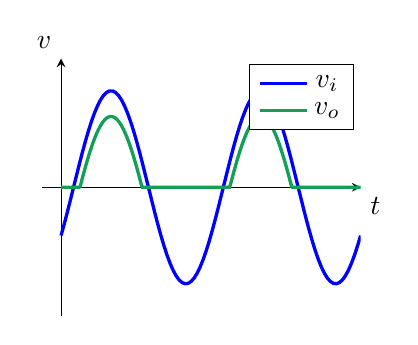
\begin{tikzpicture}
		\begin{axis}[
				axis lines = middle,
				xlabel = $t$,
				ylabel = $v$,
				xmin=-0.125,
				ymin=-1,
				xmax=2,
				ymax=1,
				xtick={0},
				ytick={0},
				xticklabels={0},
				yticklabels={0},
				xlabel style={below right},
				ylabel style={above left},
				% grid=both,
				% minor tick num=1,
				% width=0.8\textwidth,
				height=0.4\textwidth,
			]
			\addplot[domain=0:2, samples=100, blue, very thick] {0.75*sin(deg(x*2*pi-pi/6))};
			\addlegendentry{$v_i$};
			\addplot[domain=0:2, samples=300, darkgreen, very thick] {max(0,0.75*sin(deg(x*2*pi-pi/6))-0.2)};
			\addlegendentry{$v_o$};
		\end{axis}
	\end{tikzpicture}
\end{figure}

\subsection{Full-Wave Rectifier}

\begin{figure}[H]
	\centering
	\begin{circuitikz}[american]
		\ctikzset{diodes/scale=0.5}
		\ctikzset{transformer L2/.style={inductors/coils=7, inductors/width=1.0}}
		\ctikzset{transformer L1/.style={inductors/coils=7, inductors/width=1.0}}
		\ctikzset{inductors/scale=1.5}
		\draw (0,0) node[transformer core, cute] (T) {};
		\draw (T.A1) to[open, v=$v_S$, o-o] (T.A2);
		\draw (T.B1) to[diode, l_=D1] ++(1,0) coordinate (A) to[short, -o] ++(1.5,0) coordinate (B);
		\draw let \p1=(B), \p2=(T-L2.midtap) in (T-L2.midtap) to[short, -o] (\x1,\y2) to[open, v<=$v_o$] (B);
		\draw let \p1=(B), \p2=(T-L2.midtap) in (B) ++(-0.5,0) to[R, l_=$R$, *-*] ++(0,-\y1+\y2) node[ground] {};
		\draw (T.B2) to[diode, l_=D2] ++(1,0) to[short, -*] (A);
	\end{circuitikz}
\end{figure}

\begin{figure}[H]
	\centering
	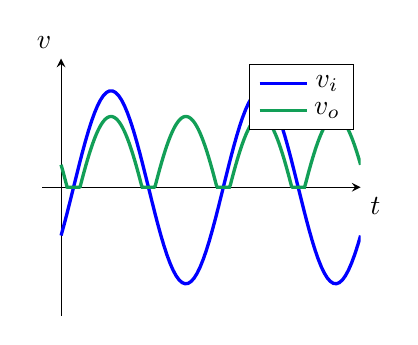
\begin{tikzpicture}
		\begin{axis}[
				axis lines = middle,
				xlabel = $t$,
				ylabel = $v$,
				xmin=-0.125,
				ymin=-1,
				xmax=2,
				ymax=1,
				xtick={0},
				ytick={0},
				xticklabels={0},
				yticklabels={0},
				xlabel style={below right},
				ylabel style={above left},
				% grid=both,
				% minor tick num=1,
				% width=0.8\textwidth,
				height=0.4\textwidth,
			]
			\addplot[domain=0:2, samples=100, blue, very thick] {0.75*sin(deg(x*2*pi-pi/6))};
			\addlegendentry{$v_i$};
			\addplot[domain=0:2, samples=300, darkgreen, very thick] {max(0,abs(0.75*sin(deg(x*2*pi-pi/6)))-0.2)};
			\addlegendentry{$v_o$};
		\end{axis}
	\end{tikzpicture}
\end{figure}

\[
	\text{PIV} = 2V_S - V_D
	.\]

\subsection{The Bridge Rectifier}

The difference between the bridge rectifier and the full-wave rectifier is that the bridge rectifier does not require a center-tapped transformer and requires more turn on voltage $2V_D$.

\begin{figure}[H]
	\centering
	\begin{circuitikz}[american]
		\ctikzset{diodes/scale=0.5}
		\ctikzset{transformer L2/.style={inductors/coils=7, inductors/width=1.0}}
		\ctikzset{transformer L1/.style={inductors/coils=7, inductors/width=1.0}}
		\ctikzset{inductors/scale=1.5}
		\draw (0,0) node[transformer core, cute] (T) {};
		\draw (T.A1) to[open, v=$v_S$, o-o] (T.A2);
		\draw (T.B1) to[short, -*] ++(2,0) coordinate (top);
		\draw (T.B2) to[short, -*] ++(2,0) coordinate (bottom);
		\coordinate (M) at ($(top)!0.5!(bottom)$);
		\draw (top) to[diode, l_=$\text{D}_4$, -*, invert] ($ (M) + (-1.5,0) $);
		\draw (top) to[diode, l^=$\text{D}_1$, -*] ($ (M) + (1.5,0) $);
		\draw (bottom) to[diode, l_=$\text{D}_3$, -*] ($ (M) + (1.5,0) $);
		\draw (bottom) to[diode, l^=$\text{D}_2$, -*, invert] ($ (M) + (-1.5,0) $);
		\draw ($ (M) + (-1.5,0) $) to[R, v^<=$v_o$, l_=$R$] ($ (M) + (1.5,0) $);
		\draw ($ (M) + (-1.5,0) $) -- ++(-0.25,0) node[ground] {};
	\end{circuitikz}
\end{figure}

\begin{figure}[H]
	\centering
	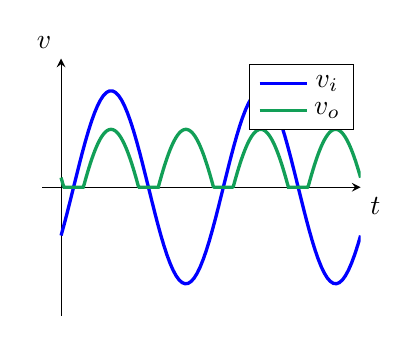
\begin{tikzpicture}
		\begin{axis}[
				axis lines = middle,
				xlabel = $t$,
				ylabel = $v$,
				xmin=-0.125,
				ymin=-1,
				xmax=2,
				ymax=1,
				xtick={0},
				ytick={0},
				xticklabels={0},
				yticklabels={0},
				xlabel style={below right},
				ylabel style={above left},
				% grid=both,
				% minor tick num=1,
				% width=0.8\textwidth,
				height=0.4\textwidth,
			]
			\addplot[domain=0:2, samples=100, blue, very thick] {0.75*sin(deg(x*2*pi-pi/6))};
			\addlegendentry{$v_i$};
			\addplot[domain=0:2, samples=300, darkgreen, very thick] {max(0,abs(0.75*sin(deg(x*2*pi-pi/6)))-0.3)};
			\addlegendentry{$v_o$};
		\end{axis}
	\end{tikzpicture}
\end{figure}


\[
	\text{PIV} = V_S - V_D
	.\]

\chapter{BJTs}

A BJT is a Bipolar Junction Transistor. It is a current controlled device. It has three terminals: the base, the collector, and the emitter. The BJT is a three-layer, two-junction semiconductor device.

\begin{figure}[H]
	\centering
	\begin{circuitikz}
		\draw (0,0) node[npn] (npn) {};
		\draw (npn.base) node[anchor=east] {B};
		\draw (npn.collector) node[anchor=south] {C};
		\draw (npn.emitter) node[anchor=north] {E};
		\draw (npn.center) ++(0,-2) node[below] {npn BJT};

		\draw (3,0) node[pnp] (pnp) {};
		\draw (pnp.base) node[anchor=east] {B};
		\draw (pnp.collector) node[anchor=north] {C};
		\draw (pnp.emitter) node[anchor=south] {E};
		\draw (pnp.center) ++(0,-2) node[below] {pnp BJT};
	\end{circuitikz}
\end{figure}

\section{BJT Current-Voltage Relationships in the Active Mode}

\begin{table}[H]
	\centering
	\renewcommand{\arraystretch}{2}
	\everymath{\displaystyle}
	\begin{tabular}{|c|c|c|}
		\hline
		\textbf{npn Transistor}             & \textbf{pnp Transistor}             & \textbf{Global}                     \\
		\hline
		$i_C = I_S e^{\sfrac{v_{BE}}{V_T}}$ & $i_C = I_S e^{\sfrac{v_{EB}}{V_T}}$ & $i_E = i_C + i_B$                   \\
		$i_B = \frac{i_C}{\beta}$           & $i_B = \frac{i_C}{\beta}$           & $\alpha = \frac{\beta}{\beta + 1}$  \\
		$i_E = \frac{i_C}{\alpha}$          & $i_E = \frac{i_C}{\alpha}$          & $\beta = \frac{\alpha}{1 - \alpha}$ \\
		\hline
	\end{tabular}
\end{table}

\section{BJT in DC}

\begin{enumerate}
	\ii Cut-off mode:
	\begin{itemize}
		\ii $i_E = i_C = i_B = 0$
		\ii $v_{BE} < \SI{0.5}{\volt}$ and $v_{BC} < \SI{0.4}{\volt}$
	\end{itemize}

	\ii Saturation mode:
	\begin{itemize}
		\ii $v_{BE} = \SI{0.7}{\volt}$ and $i_B : i_C : i_E = 1 : \beta : \beta + 1$
		\ii $v_{CE} > \SI{0.3}{\volt}$
	\end{itemize}

	\ii Active mode:
	\begin{itemize}
		\ii $v_{BE} = \SI{0.7}{\volt}$ and $v_{CE} = \SI{0.2}{\volt}$
		\ii $\sfrac{i_C}{i_B} = \beta_\text{forced} < \beta$
	\end{itemize}
\end{enumerate}

\section{Small Signal Model of a BJT}

The transconductance of a BJT is given by

\[
	g_m = \eval{ \pdv{i_C}{ v_{BE} } }_{i_C=I_C} = \frac{I_C}{V_T}
	.\]

\begin{align*}
	r_\pi & = \frac{\beta}{g_m} = \frac{V_T}{I_B}  \\
	r_e   & = \frac{\alpha}{g_m} = \frac{V_T}{I_E} \\
	r_0   & = \frac{V_A}{I_C}
\end{align*}

\subsection{The Hybrid-$\pi$ Model}

\begin{figure}[H]
	\centering
	\begin{circuitikz}[american]
		\draw (0,0) node[left] {B}
		to[short, o-] ++(1,0)
		to[R, l=$r_\pi$, v_>=$v_{be}$] ++(0,-2) coordinate (A)
		to[short] ++(3,0)
		to[cI, l=$g_m v_{be}$, invert] ++(0,2)
		to[short, -o] ++(1,0) node[right] {C};

		\draw (A) ++(1.5,0) to[short, *-o] ++(0,-1) node[below] {E};

		\draw (8,0) node[left] {B}
		to[short, o-] ++(1,0)
		to[R, l=$r_\pi$, v_>=$v_{be}$] ++(0,-2) coordinate (B)
		to[short] ++(3,0)
		to[cI, l=$g_m v_{be}$, invert] ++(0,2)
		to[short, -o] ++(2,0) node[anchor=west] {C}
		++(-1,0)
		to[R=$r_0$, *-] ++(0,-2)
		to[short, -*] ++(-1,0);

		\draw (B) ++(1.5,0) to[short, *-o] ++(0,-1) node[below] {E};
	\end{circuitikz}
\end{figure}

\begin{figure}[H]
	\centering
	\begin{circuitikz}[american]
		\draw (0,0) node[left] {B}
		to[short, o-] ++(1,0)
		to[R, l=$r_\pi$, i_>=$i_{b}$] ++(0,-2) coordinate (A)
		to[short] ++(3,0)
		to[cI, l=$\beta i_{b}$, invert] ++(0,2)
		to[short, -o] ++(1,0) node[right] {C};

		\draw (A) ++(1.5,0) to[short, *-o] ++(0,-1) node[below] {E};

		\draw (8,0) node[left] {B}
		to[short, o-] ++(1,0)
		to[R, l=$r_\pi$, i_>=$i_{b}$] ++(0,-2) coordinate (B)
		to[short] ++(3,0)
		to[cI, l=$\beta i_{b}$, invert] ++(0,2)
		to[short, -o] ++(2,0) node[anchor=west] {C}
		++(-1,0)
		to[R=$r_0$, *-] ++(0,-2)
		to[short, -*] ++(-1,0);

		\draw (B) ++(1.5,0) to[short, *-o] ++(0,-1) node[below] {E};
	\end{circuitikz}
\end{figure}

\subsection{The T Model}

\begin{figure}[H]
	\centering
	\begin{circuitikz}[american]
		\draw (0,0) node[above] {C} to[short,o-] ++(0,-0.5) coordinate (A) to[cI, l=$g_m v_{be}$] ++(0,-2) coordinate (B) to[R=$r_e$, v_=$v_{be}$] ++(0,-2) coordinate (C) to[short,-o] ++(0,-0.5) node[below] {E};
		\draw (B) to[short,*-o] ++(-2,0) node[left] {B};

		\draw (5,0) node[above] {C} to[short,o-] ++(0,-0.5) coordinate (A) to[cI, l=$g_m v_{be}$] ++(0,-2) coordinate (B) to[R=$r_e$, v_=$v_{be}$] ++(0,-2) coordinate (C) to[short,-o] ++(0,-0.5) node[below] {E};
		\draw (B) to[short,*-o] ++(-2,0) node[left] {B};
		\draw (A) to[short] ++(2,0) to[short] ++(0,-1) to[R=$r_0$] ++(0,-2) to[short] ++(0,-1) to[short] (C);
	\end{circuitikz}
\end{figure}

\begin{figure}[H]
	\centering
	\begin{circuitikz}[american]
		\draw (0,0) node[above] {C} to[short,o-] ++(0,-0.5) coordinate (A) to[cI, l=$\alpha i_e$] ++(0,-2) coordinate (B) to[R=$r_e$, i_=$i_e$] ++(0,-2) coordinate (C) to[short,-o] ++(0,-0.5) node[below] {E};
		\draw (B) to[short,*-o] ++(-2,0) node[left] {B};

		\draw (5,0) node[above] {C} to[short,o-] ++(0,-0.5) coordinate (A) to[cI, l=$\alpha i_e$] ++(0,-2) coordinate (B) to[R=$r_e$, i_=$i_e$] ++(0,-2) coordinate (C) to[short,-o] ++(0,-0.5) node[below] {E};
		\draw (B) to[short,*-o] ++(-2,0) node[left] {B};
		\draw (A) to[short] ++(2,0) to[short] ++(0,-1) to[R=$r_0$] ++(0,-2) to[short] ++(0,-1) to[short] (C);
	\end{circuitikz}
\end{figure}


\chapter{MOSFETs}

A MOSFET is a Metal Oxide Semiconductor Field Effect Transistor. It is a voltage controlled device.

It has three terminals: the gate, the source, and the drain.

\begin{figure}[H]
	\centering
	\begin{circuitikz}
		\ctikzset{tripoles/mos style/arrows}
		\draw (0,0) node[nmos] (mos) {};
		\draw (mos.gate) node[anchor=east] {G};
		\draw (mos.source) node[anchor=north] {S};
		\draw (mos.drain) node[anchor=south] {D};
	\end{circuitikz}
\end{figure}

\section{MOSFET Modes of Operation}

\nt{
	\[
		k_n = \mu_n C_{ox} \frac{W}{L} \\
		.\]
}

\begin{figure}[H]
	\centering
	\begin{circuitikz}
		\ctikzset{tripoles/mos style/arrows}
		\draw (0,0) node[nmos] (mos) {};
		\draw (mos.gate) node[anchor=east] {G};
		\draw (mos.source) node[anchor=north] {S};
		\draw (mos.drain) node[anchor=south east] {D};
		\draw (mos.gate) to[open, v=$v_{GS}$] (mos.source);
		\draw (mos.drain) to[short, i_=$i_D$] ++(0,0.5);
		\draw (mos.drain) to[open, v^=$v_{DS}$] (mos.source);
	\end{circuitikz}
\end{figure}

\subsection{Cut-off}

In this mode, the MOSFET is off ($i_D = 0$). The MOSFET is in cut-off when $v_{GS} \leq V_{th}$. Where $V_{th}$ is the threshold voltage of the MOSFET.\\


\subsection{Triode}

In this mode, the MOSFET is on ($i_D \neq 0$). The MOSFET conducts current from the drain to the source. The MOSFET is in triode when $v_{GS} > V_{th}$ and $v_{DS} < v_{GS} - V_{th}$.

\[
	i_D = \mu_n C_{ox} \frac{W}{L} \left[ (v_{GS} - V_{th}) v_{DS} - \frac{v_{DS}^2}{2} \right]
	.\]


\subsection{Saturation}

In this mode, the MOSFET is on ($i_D \neq 0$). The MOSFET conducts current from the drain to the source. The MOSFET is in saturation when $v_{GS} > V_{th}$ and $v_{DS} > v_{GS} - V_{th}$.

\[
	i_D = \frac{1}{2} \mu_n C_{ox} \frac{W}{L} (v_{GS} - V_{th})^2
	.\]

\section{Small Signal Model of a MOSFET}

\begin{align*}
	g_m & = \frac{2 I_D}{V_{GS} - V_{th}}           \\
	r_o & = \frac{V_A}{I_D} = \frac{1}{\lambda I_D}
\end{align*}

\subsection{The Hybrid-$\pi$ Model}

\begin{figure}[H]
	\centering
	\begin{circuitikz}
		\draw (-2,0) node (G1) {} node[left] {G} to[short, o-o] ++(0.5,0);
		\draw (-2,-3) node (G2) {} to[short, o-o] ++(5,0) node (D2) {};
		\draw (2.5, -3) to[short, *-o] ++(0,-0.5) node[below] {S};
		\draw (3.5,-3) to[american, cisource, invert, *-, l=$g_m v_{gs}$] ++(0,3) to [short, -o] ++(1.5,0) node (D1) {} node[right] {D};

		\draw (G1) to[american, open, v=$v_{GS}$] (G2);
		\draw (D1) to[american, open, v^=$v_{DS}$] (D2);

		\begin{scope}[xshift=8cm]
			\draw (-2,0) node (G1) {} node[left] {G} to[short, o-o] ++(0.5,0);
			\draw (-2,-3) node (G2) {} to[short, o-o] ++(8,0) node (D2) {};
			\draw (2.5, -3) to[short, *-o] ++(0,-0.5) node[below] {S};
			\draw (3.5,-3) to[american, cisource, invert, *-, l=$g_m v_{gs}$] ++(0,3) to [short, -o] ++(2.5,0) node (D1) {} node[right] {D};
			\draw (4.5, 0) to[R=$r_o$, *-*] ++(0,-3);

			\draw (G1) to[american, open, v=$v_{GS}$] (G2);
			\draw (D1) to[american, open, v^=$v_{DS}$] (D2);
		\end{scope}
	\end{circuitikz}
\end{figure}


\begin{figure}[H]
	\centering
	\begin{circuitikz}
	\end{circuitikz}
\end{figure}

\subsection{The T Model}

\begin{figure}[H]
	\centering
	\begin{circuitikz}[american]
		\draw (0,0) node[above] {D}
		to[short,o-] ++(0,-0.5) coordinate (A)
		to[cI, l=$1 \times i$] ++(0,-2) coordinate (B)
		to[R=$\frac{1}{g_m}$, i_=$i$] ++(0,-2) coordinate (C)
		to[short,-o] ++(0,-0.5) node[below] {S};
		\draw (B) to[short,*-o] ++(-2,0) node[left] {G};

		\draw (5,0) node[above] {D}
		to[short,o-] ++(0,-0.5) coordinate (A)
		to[cI, l=$1 \times i$] ++(0,-2) coordinate (B)
		to[R=$\frac{1}{g_m}$, i_=$i$] ++(0,-2) coordinate (C)
		to[short,-o] ++(0,-0.5) node[below] {S};
		\draw (B) to[short,*-o] ++(-2,0) node[left] {G};
		\draw (A) to[short] ++(2,0) to[short] ++(0,-1) to[R=$r_0$] ++(0,-2) to[short] ++(0,-1) to[short] (C);
	\end{circuitikz}
\end{figure}

\chapter{Operational Amplifiers}

An operational amplifier is a high gain differential amplifier. It has two inputs: the inverting input and the non-inverting input. It has one output.

\section{Inverting Configuration}

\begin{figure}[H]
	\centering
	\begin{circuitikz}[american]
		\draw (0,0) node[op amp] (opamp) {};
		\draw (opamp.+) to[short] ++(-0.5,0) node[ground] {};
		\draw (opamp.-) to[R, l_=$R_1$, -o] ++(-2,0) to[short] ++(-1,0) to[sV, l=$v_i$] ++(0,-1.25) node[ground] {};
		\draw (opamp.-) to[short, *-] ++(0,1) to[R=$R_f$] ++(2,0) -| (opamp.out);
		\draw (opamp.out) to[short, *-o] ++(1,0) node[right] {$\displaystyle v_o = -\frac{R_f}{R_1}v_i$};
	\end{circuitikz}
\end{figure}

\begin{figure}[H]
	\centering
	\begin{circuitikz}[american]
		\draw (0,0) node[op amp] (opamp) {};
		\draw (opamp.+) to[short] ++(-0.5,0) node[ground] {};
		\draw (opamp.-) to[R, l_=$R_1$, -o] ++(-2,0) to[short] ++(-1,0) to[sV, l=$v_i$] ++(0,-1.25) node[ground] {};
		\draw (opamp.-) to[short, *-] ++(0,2.5) to[R=$R_2$,-*] ++(2,0) coordinate (A) to[R=$R_4$] ++(2,0) |- (opamp.out);
		\draw (A) to[R=$R_3$] ++(0,-2) node[ground] {};
		\draw (opamp.out) to[short, *-o] ++(2,0) node[right] {$\displaystyle v_o = -\frac{R_2}{R_1}\lt( 1 + \frac{R_4}{R_2} + \frac{R_4}{R_3} \rt) v_i$};
	\end{circuitikz}
\end{figure}

\subsection{The Summing Amplifier}

\begin{figure}[H]
	\centering
	\begin{circuitikz}[american]
		\draw (0,0) node[op amp] (opamp) {};
		\draw (opamp.+) to[short] ++(-0.5,0) node[ground] {};
		\draw (opamp.-) to[short] ++(-2,0) coordinate (A);
		\draw (A) to[short] ++(0,1) to[R=$R_1$,-o] ++(-2,0) node[left] {$v_1$};
		\draw (A) to[short] ++(0,0) to[R=$R_2$,-o] ++(-2,0) node[left] {$v_2$};
		\draw (A) to[short] ++(0,-1) to[R=$R_n$,-o] ++(-2,0) node[left] {$v_n$};
		\draw (opamp.-) to[short, *-] ++(0,1) to[R=$R_f$] ++(2,0) -| (opamp.out);
		\draw (opamp.out) to[short, *-o] ++(1,0) node[right] {$\displaystyle v_o = -R_f\lt( \frac{1}{R_1}v_1 + \frac{1}{R_2}v_2 + \cdots + \frac{1}{R_n}v_n \rt)$};
	\end{circuitikz}
\end{figure}

\section{Non-Inverting Configuration}

\begin{figure}[H]
	\centering
	\begin{circuitikz}[american]
		\draw (0,0) node[op amp] (opamp) {};
		\draw (opamp.+) to[short, o-] ++(-0.5,0) to[sV, l=$v_i$] ++(0,-1.5) node[ground] {};
		\draw (opamp.-) to[R, l_=$R_1$, -o] ++(-2,0) node[ground] {};
		\draw (opamp.-) to[short, *-] ++(0,1) to[R=$R_f$] ++(2,0) -| (opamp.out);
		\draw (opamp.out) to[short, *-o] ++(1,0) node[right] {$\displaystyle v_o = \lt( 1 + \frac{R_f}{R_1} \rt)v_i$};
	\end{circuitikz}
\end{figure}

\section{Difference Amplifier}

\begin{figure}[H]
	\centering
	\begin{circuitikz}[american]
		\draw (0,0) node[op amp] (opamp) {};
		\draw (opamp.+) to[R=$R_4$] ++(0,-1.5) node[ground] {};
		\draw (opamp.+) to[R=$R_3$,*-o] ++(-2,0) node[left] {$v_{I2}$};
		\draw (opamp.-) to[R, l_=$R_1$, -o] ++(-2,0) node[left] {$v_{I1}$};
		\draw (opamp.-) to[short, *-] ++(0,1) to[R=$R_f$] ++(2,0) -| (opamp.out);
		\draw (opamp.out) to[short, *-o] ++(1,0) node[right] {$\displaystyle v_o = \lt( 1 + \frac{R_f}{R_1} \rt)v_i$};
	\end{circuitikz}
\end{figure}

\section{Integrator}

\begin{figure}[H]
	\centering
	\begin{circuitikz}[american]
		\draw (0,0) node[op amp] (opamp) {};
		\draw (opamp.+) to[short] ++(-0.5,0) node[ground] {};
		\draw (opamp.-) to[R, l_=$R$, -o] ++(-2,0) to[short] ++(-1,0) to[sV, l=$v_i$] ++(0,-1.25) node[ground] {};
		\draw (opamp.-) to[short, *-] ++(0,1.5) to[C,l_=$C$, v^=$v_C$] ++(2,0) -| (opamp.out);
		\draw (opamp.out) to[short, *-o] ++(1,0) node[right] {$\displaystyle v_o = -\frac{1}{RC}\int_0^t\!v_i(t)\dd{t} - V_C$};
	\end{circuitikz}
\end{figure}

\section{Differentiator}

\begin{figure}[H]
	\centering
	\begin{circuitikz}[american]
		\draw (0,0) node[op amp] (opamp) {};
		\draw (opamp.+) to[short] ++(-0.5,0) node[ground] {};
		\draw (opamp.-) to[C=$C$, -o] ++(-2,0) to[short] ++(-1,0) to[sV, l=$v_i$] ++(0,-1.25) node[ground] {};
		\draw (opamp.-) to[short, *-] ++(0,1) to[R=$R$] ++(2,0) -| (opamp.out);
		\draw (opamp.out) to[short, *-o] ++(1,0) node[right] {$\displaystyle v_o = -RC\dv{v_i(t)}{t}$};
	\end{circuitikz}
\end{figure}

\end{document}
